\documentclass{article}

% Packages
\usepackage[utf8]{inputenc}

\usepackage{amsmath, bm}
\usepackage{graphicx}
\usepackage{amssymb}
\usepackage{float}
\usepackage{caption}
\usepackage{subcaption}
\usepackage{geometry}

\newgeometry{vmargin={1in}, hmargin={1in}}


\title{3A1 Transition to Turbulence Lab Report}
\author{[Louis Pender]}
\date{February 29, 2024}

\begin{document}

\maketitle

\section{Introduction}



\section{Theory}
% Describe the experimental setup, equipment used, and the steps followed during the experiment.

\subsection{Hot wire anemometry}

The hot wire anemometer is a device used to measure the velocity of a fluid.
The wires resistance changes with temperature and the convective heat loss is related to the velocity of the fluid.
This is measured by a Wheatstone bridge circuit which is balanced at a constant temperatue.
The heat loss of the wire can be modelled by King's Law
\begin{equation}
    E^2 = A + B U^{\frac{1}{2}}
\end{equation}
Considering a turbulent flow the velocity profile can be modelled as a mean velocity $\bar{U} + u'$ where $u'$ is the fluctuating component.
The voltage then can also be modelled as a mean voltage $\bar{E} + e'$ where $e'$ is the fluctuating component.



%%%%%%%%%%%%%%%%%%%%

\section{Results}
% Present the data obtained from the experiment, including tables, graphs, and figures.

The density of air $\rho = 1.225kgm^{-3}$ for the standard atmosphere with 15oC and 760 mmHg

\begin{figure}[H]
    \centering
    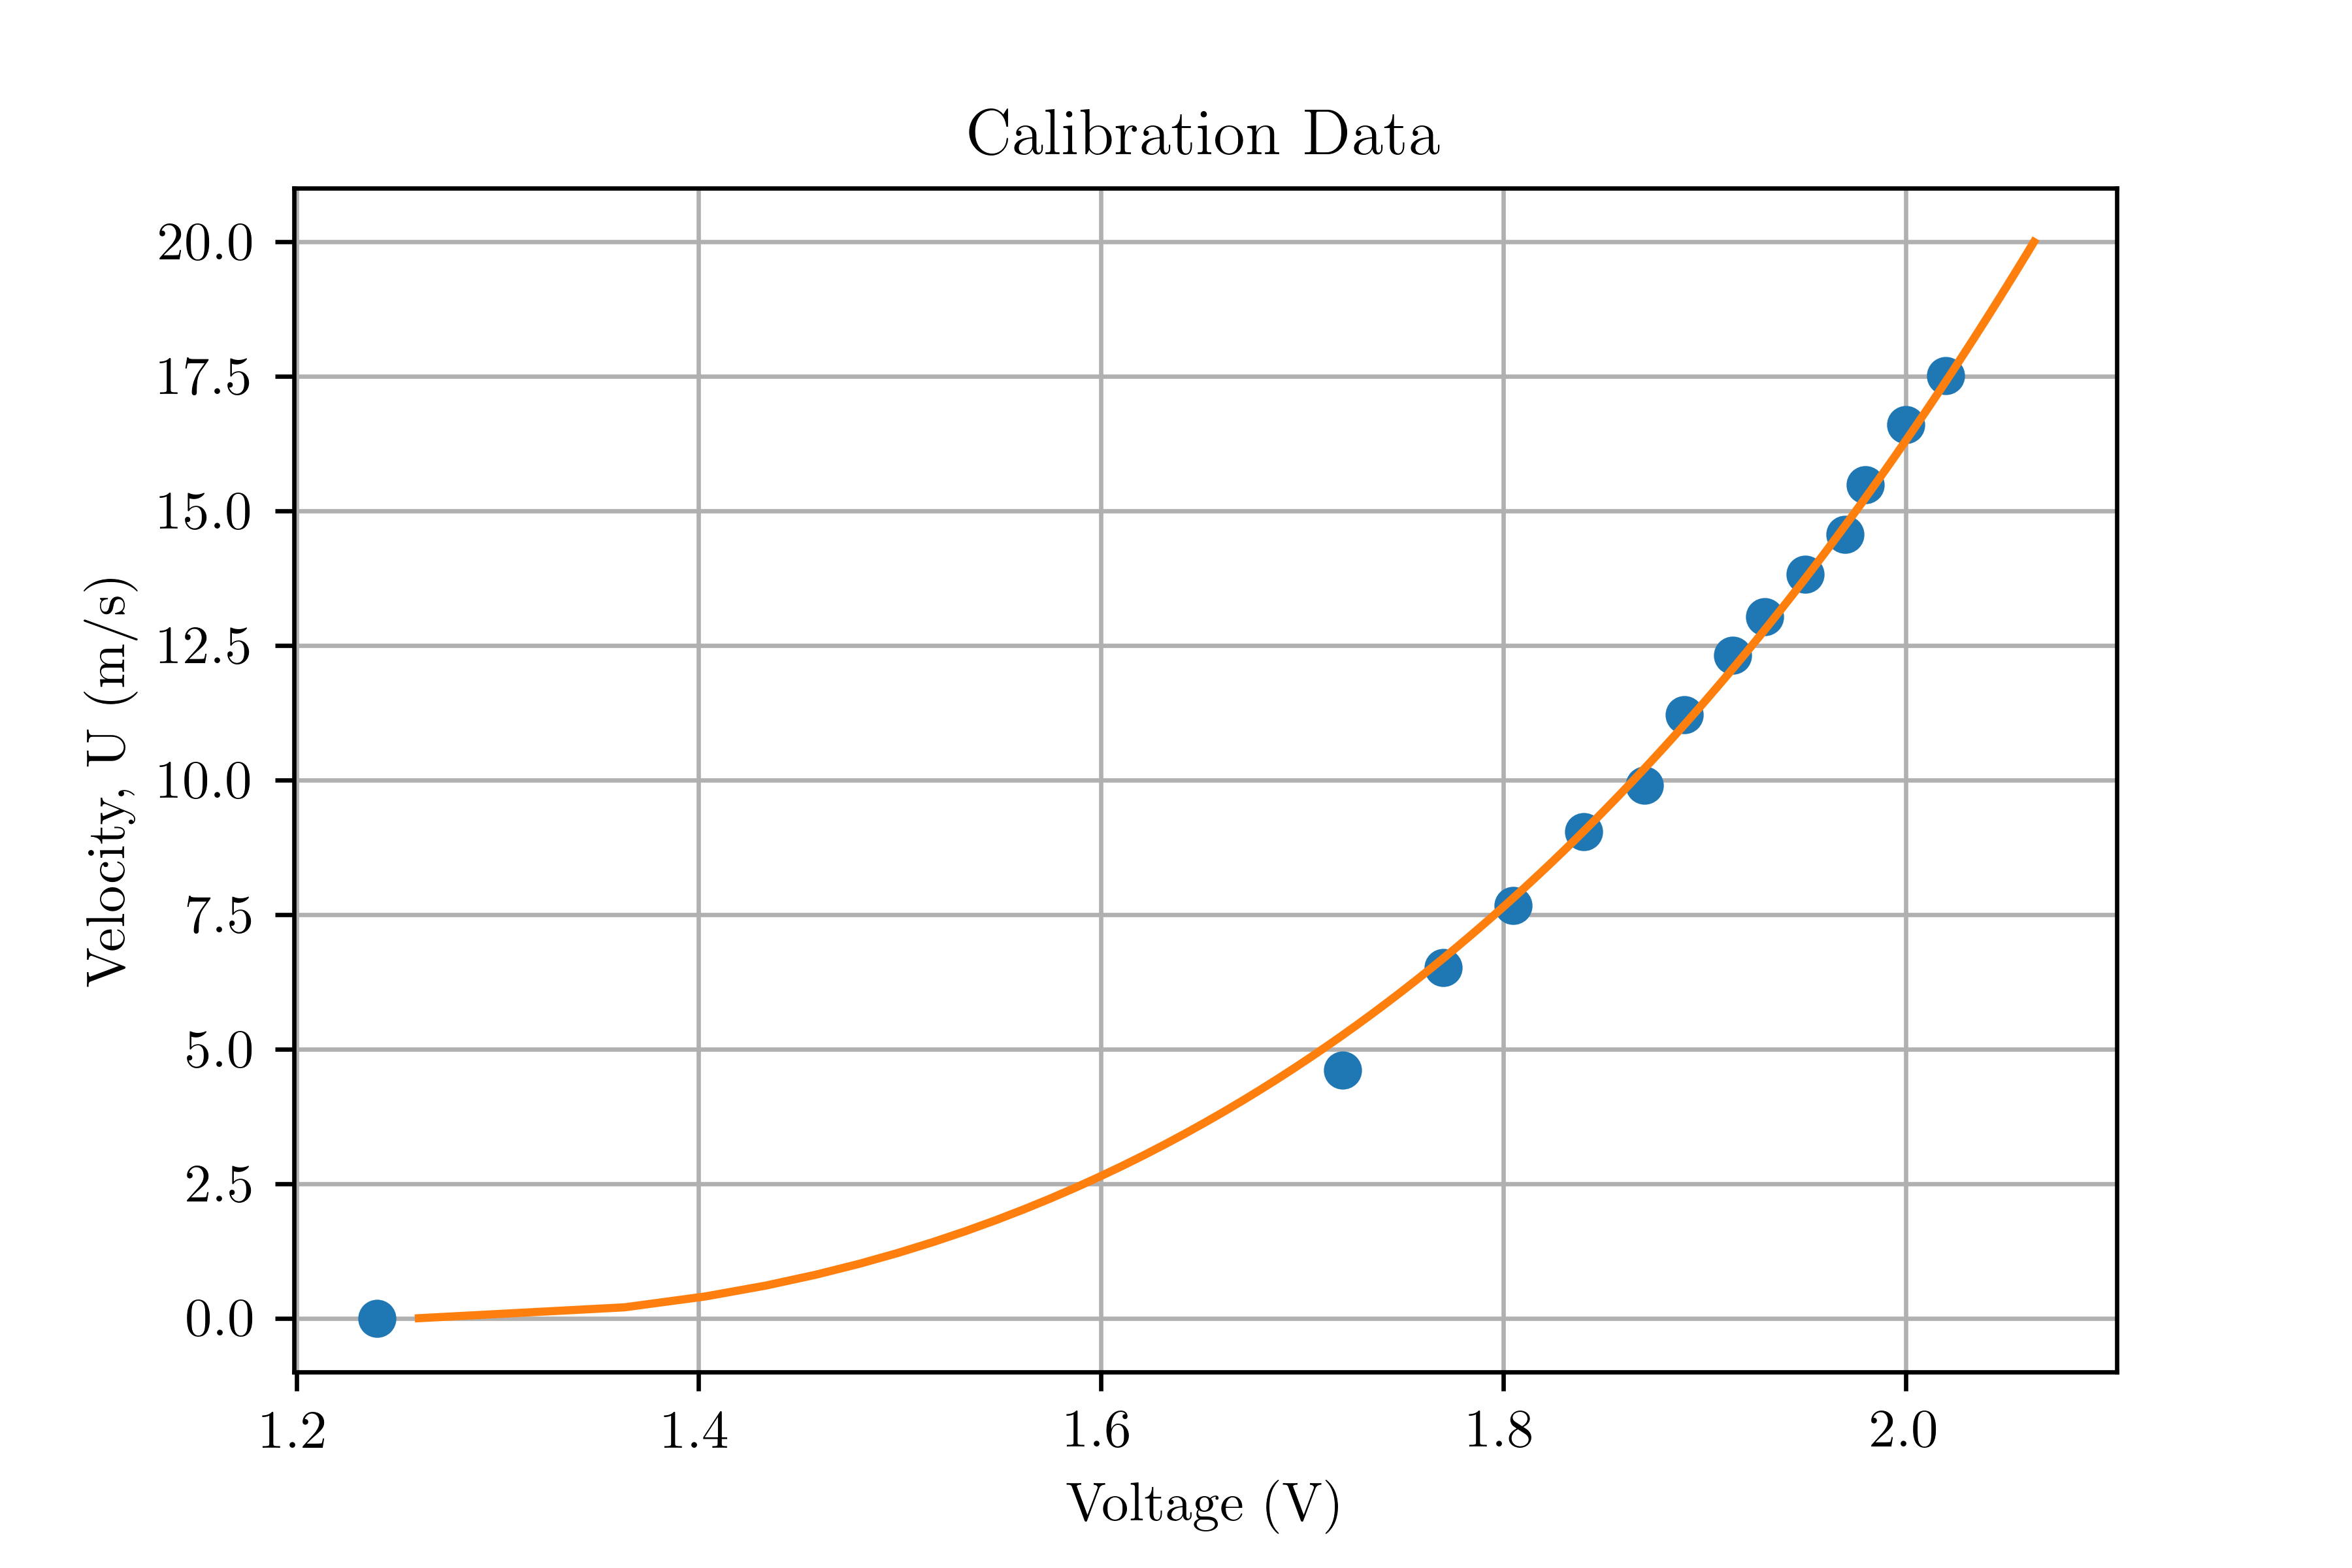
\includegraphics[width=0.8\textwidth]{calibration.png}
    \caption{Calibration curve for the hot wire anemometer}
    \label{fig:calibration}
\end{figure}



% 1. Express your results in terms of the Reynolds number.



%%%%%%%%%%%%%%%%%%%%%%%

\section{Discussion}
% Analyze and interpret the results, discussing their significance and any observations or trends.


% 2. Discuss the observations you have made.

% laminar boundary layer

% 3. How long are the intermittent patches of turbulence (spots) in the transition zone?

% 4. Try to estimate the size of a typical eddy in the turbulent flow.

% 5. For the boundary layer profile, calculate the velocity ratio u'/U1
% where u'(y) is the velocity at height y and U1 ( is the free-stream velocity, and plot versus y, the distance
% from the surface. The points should also be plotted on the Clauser plot supplied. The
% demonstrator will provide you with the zero offset when the probe stop is just in
% contact with the plate (≈ 0.2mm).

The linear region on the Clauser plot should provide an estimation of the skin friction Cf.
Calculate the friction velocity
\begin{equation}
    U_* = \left( \frac{\tau}{\rho} \right)^{\frac{1}{2}} = \left[ \frac{1}{2}C_f \bar{ U}_1^2 \right]^{\frac{1}{2}}
\end{equation}


% 7. Calculate and plot versus distance from the wall on separate axes and discuss


\section{Conclusion}
% Summarize the main findings of the experiment and draw conclusions based on the results.


%%%%%%%%%%%%%%%%%%%%%%%

\section{Appendix}

\begin{figure}[H]
    \centering
    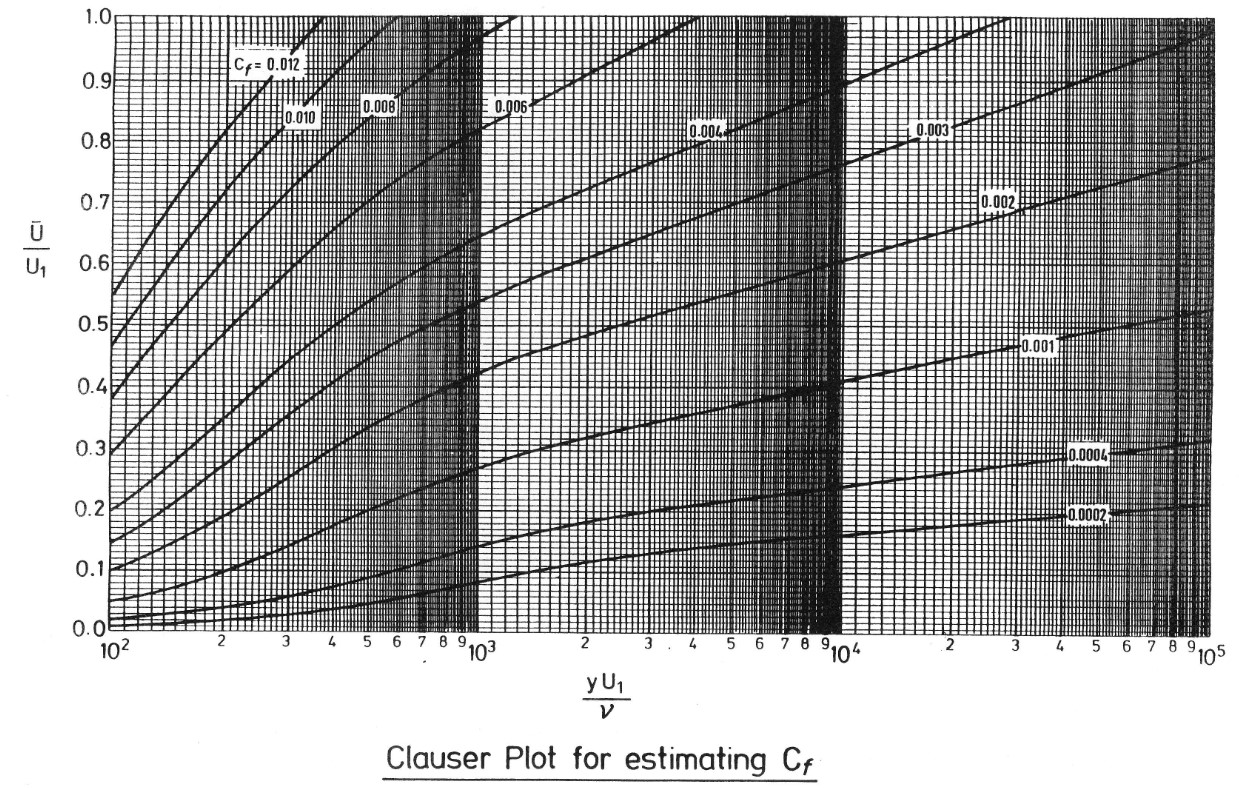
\includegraphics[width=0.8\textwidth]{clauser.jpg}
    \caption{Clauser plot}
    \label{fig:clauser}
\end{figure}

\begin{thebibliography}{9}
    \bibitem{handout}
    Cambridge University Engineering Department, \textit{Module 3A1: Transition to Turbulence Lab handout}
\end{thebibliography}

\end{document}
